% \documentclass{beamer}
\documentclass[aspectratio=169]{beamer}
\usepackage{hyperref}
%% \usepackage[CJKmath=true, AutoFakeBold = true]{xeCJK}
\usepackage[T1]{fontenc}
%% \setCJKmainfont{AR PL KaitiM GB} % Set Chinese font to KaiTi (calligraphy style)

% Other packages
\usepackage{latexsym,xcolor,multicol,booktabs,calligra}
% \usepackage{amssymb,amsfonts,amsmath,amsthm,mathrsfs,mathptmx} % Common math packages
\usepackage{amsmath,amssymb,amsfonts,mathrsfs} % Best mathematical packages
\usepackage{newtxtext,newtxmath} % Times-like font package for text and mathematics

\usepackage{graphicx,pstricks,listings,stackengine}
\usefonttheme[onlymath]{serif} % Use serif font for equations (better appearance)

% Other packages (new)
\usepackage[linesnumbered,ruled,vlined]{algorithm2e}
\SetKwComment{Comment}{$\triangleright$ }{} % The argument will be surrounded by /* ... */
\SetAlCapFnt{\footnotesize} % Make caption text smaller
\SetAlCapNameFnt{\footnotesize} % Make "Algorithm" label smaller
\usepackage{graphicx} % Enables inclusion and scaling of images (\includegraphics)
\usepackage{animate} % Provides support for frame-by-frame animations (\animategraphics)
\usepackage{subcaption} % Provides support for subfigures (subfigure environment with captions)
\usepackage{fontawesome5} % Provides scalable vector icons (Font Awesome 5 icons)
\usepackage{caption}
\captionsetup{
    font=footnotesize, % Reduce caption text size
    skip=5pt, % Space between figure and caption
    belowskip=0pt % Space below the caption (reduces gap after caption)
}
\usepackage{forest}
\usepackage[table]{xcolor}

% Adjusts horizontal margins of the slide content
% \setbeamersize{
%     text margin left=20pt, % Left margin of the slide content
%     text margin right=20pt % Right margin of the slide content
% }

\newcommand{\source}[1]{\par\tiny Source: #1} % Defines a reusable command to display the image/table source in small font below the caption

\renewcommand{\today}{\number\year-\number\month-\number\day}
\renewcommand{\alert}[1]{\textbf{\color{swufe}#1}}
\newcommand{\alertplain}[1]{{\color{swufe}#1}}

% Title page setup
\author[Alvarez-Mamani et al.]{\underline{Edwin Alvarez-Mamani} \inst{1,2}, Deybis Paucar Pinto \inst{1, 2}, Florian Buettner \inst{3}, Alfredo J. Ibañez \inst{1}, Madina Mansurova \inst{1}}
% \author[Topics]{Topics}

% Goethe-University Frankfurt and the German Cancer Consortium (DKTK)/German Cancer Research Center (DKFZ).

\title[Mass Spectrometry Data analysis via Graph Machine Learning]{Mass Spectrometry Data analysis via Graph Machine Learning}
% Custom title template with a styled box
\setbeamertemplate{title}{
    \makebox[\textwidth]{ % force horizontal centering
        \begin{beamercolorbox}[
            wd=1.0\textwidth,
            sep=1pt,
            center,
            rounded=true,
            shadow=false
        ]{title}
            \usebeamerfont{title}
            \inserttitle
        \end{beamercolorbox}
    }
}

% \subtitle{Jiangnan University Academic Report Beamer Template}
\institute[ICOBA-PUCP, IA-PUCP]{\footnotesize{\inst{1} Institute for Omics Sciences and Applied Biotechnology, Pontificia Universidad Católica del Perú} \\ \footnotesize{\inst{2} Department of Informatics, Universidad Nacional de San Antonio Abad del Cusco} \\ \footnotesize{\inst{3} German Cancer Research Center, Goethe University Frankfurt and German Cancer Consortium}}
% \institute[JNU]{\normalsize{\inst{1} School of Business \quad Jiangnan University \quad \textit{****@qq.com}}}

% \institute[ICOBA-PUCP, UNSAAC]{
%     
\includegraphics[width=0.15\linewidth]{../images/pucp.png}
% }

% \date{\today}
\date{\scriptsize June, 2026}

\usepackage{JNU}

% Defs
\def\cmd#1{\texttt{\color[RGB]{0, 0, 139}\footnotesize $\backslash$#1}}
\def\env#1{\texttt{\color[RGB]{0, 0, 139}\footnotesize #1}}

\lstset{
    language=[LaTeX]TeX,
    basicstyle=\ttfamily\footnotesize,
    keywordstyle=\bfseries\color[RGB]{0, 0, 139},
    stringstyle=\color[RGB]{50, 50, 50},
    numbers=left,
    numberstyle=\small\color{gray},
    rulesepcolor=\color{red!20!green!20!blue!20},
    frame=shadowbox,
}

\begin{document}

\begin{frame}
    \titlepage
    \begin{figure}[htpb]
        \begin{center}
            %% 
\includegraphics[width=0.55\linewidth]{../images/jiangnan_logo.png}
        \end{center}
    \end{figure}
\end{frame}

% \begin{frame}
%     \frametitle{Outline}
%     \tableofcontents[sectionstyle=show,subsectionstyle=show/shaded/hide,subsubsectionstyle=show/shaded/hide]
%     % \tableofcontents[sectionstyle=show,subsectionstyle=hide,subsubsectionstyle=hide]
% \end{frame}

% Timing: Your total presentation length is 15 minutes, broken down as:  
% - 10-12 minutes of talking/presenting 
% - 2-4 minutes of Q&A with the audience 
% - 1 minute to transition to the next speaker 

% Quitar Outline

\section{Introduction}
    \begin{frame}{Problem formulation}
        % Targeted and untargeted analyses
        The mass spectrometry analysis includes two approach: \alert{targeted} analysis and \alert{untargeted} analysis.

        % \begin{itemize}
        %     \item \alert{Targeted approach:} the molecule of interest or m/z values (for MS and MS/MS) are predefined for quantitation of analytes present in a complex samples matrix. %, with high sensitivity, accuracy, and specificity
        %     \item \alert{Untargeted approach:} is the analysis to identify the unknowns in a sample, using parent ion and product or fragment ion analysis (MS/MS).
        % \end{itemize}

        \begin{columns}[b] % Option "c" centers vertically, while "t" aligns to the top.
            \begin{column}{0.65\textwidth}
                \begin{figure}[htp!]
                    \centering
                    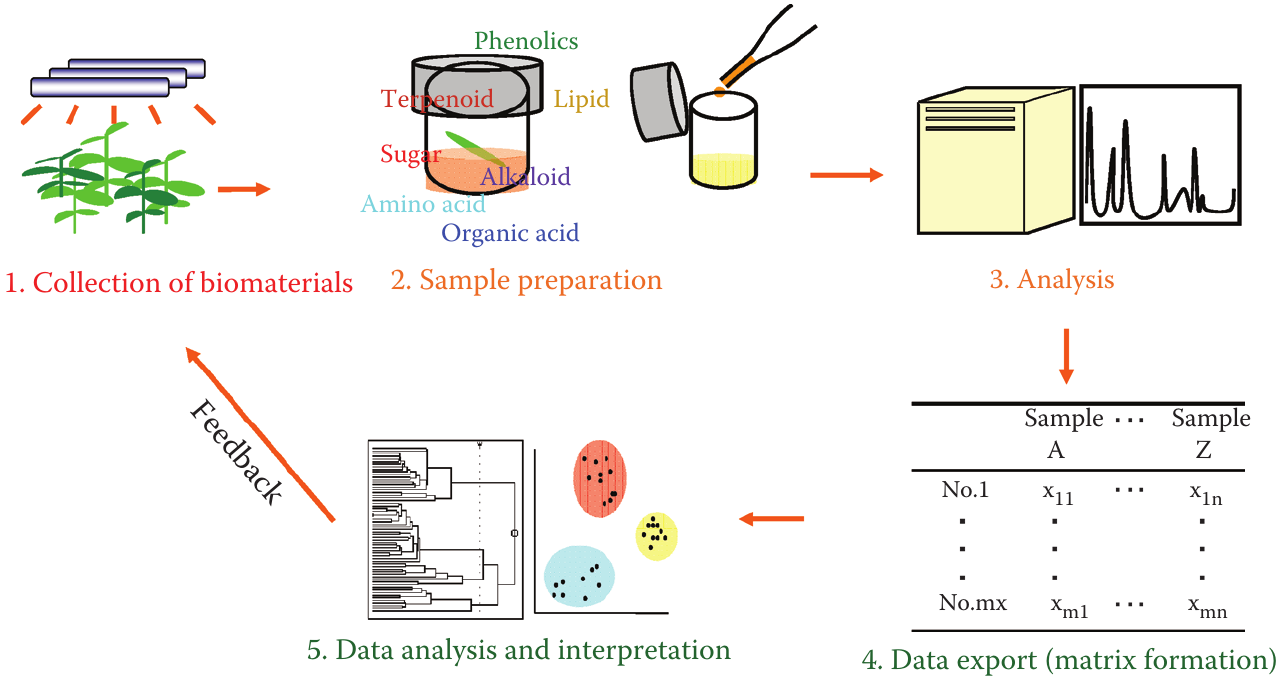
\includegraphics[
                        width=1.0\linewidth,
                        trim=0pt 0pt 0pt 0pt, % trim: left bottom right top
                        clip
                    ]{../images/metabolomics_workflow.png}
                    \caption{Metabolomics workflow.}
                    \source{\cite{putri2014mass}} 
                    % \label{fig:my_image}
                \end{figure}
            \end{column}
            \begin{column}{0.35\textwidth}
                \begin{figure}[htp!]
                    \centering
                    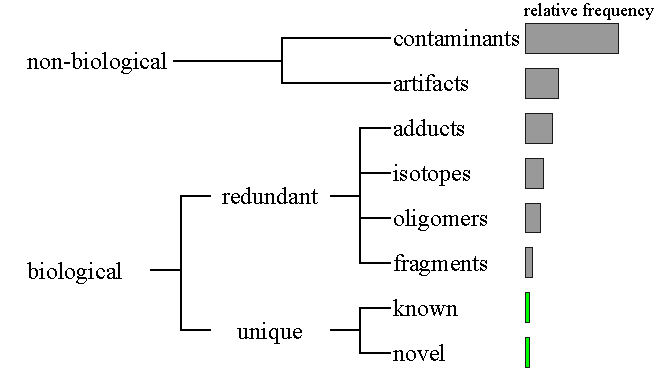
\includegraphics[
                        width=1.0\linewidth,
                        trim=0pt 0pt 0pt 0pt, % trim: left bottom right top
                        clip
                    ]{../images/untargeted_data.pdf}
                    \caption{Untargeted composition.}
                    \source{Adapted from \cite{sindelar2020chemical}}
                    % \label{fig:my_image}
                \end{figure}
            \end{column}
        \end{columns}

        \begin{note}
            {Introduce your self}
        \end{note}
    \end{frame}

    % \begin{frame}{Untargeted mass spectrometry workflow}
    %     A data matrix (sample vs. metabolites) acquired from a mass spectrometry-based metabolomics study includes not only biological information but also technical noise. % There are several techniques for univariate or multivariate statistical analysis. Some statistical methods used are: Principal component analysis (PCA), Hierarchical cluster analysis (HCA), Correlation analysis (CA), Projection to latent structure regression (PLS-R), Projection to latent structure discriminant analysis (PLS-DA), and t-Test. It is very important to use and interpret the statistical result accurate \cite{putri2014mass}.

    %     \begin{note}
    %         {Introduce your self}
    %     \end{note}
    % \end{frame}

    \begin{frame}{Our objectives}
        Filter mass spectrometry data via graph machine learning models.

        % Filtering and detecting of significant changes between metabolomic networks using graph representation learning models and an anomaly detection algorithm to obtain reliable results in less time.

        % \begin{itemize}
        %     % \item Improve the detection of significant changes between metabolomic networks using Graph Neural Network (GNN) models and to obtain reliable results in less time.
        %     % \item Develop a pipeline for data processing and analysis.
        %     % \item Develop a pipeline for data processing and analysis.

        %     \item Develop a pipeline for the analysis of metabolomic networks.
        %     \item Model metabolomic networks from mass spectrometry data.
        %     \item Implement GNN models to learn metabolite representations. % for network alignment tasks
        %     \item Evaluate the effectiveness of the proposed GNN-based alignment approach.
        %     % \item Comparison of the quality of node embeddings. % (generated by GNN models) for the analysis of metabolomic networks. % check
        %     % \item Evaluation of execution times in the generation and manipulation of embeddings.
        %     % \item Implement a web application for the analysis of metabolomic networks.
        %     % \item Develop a web application.
        % \end{itemize}

        \begin{note}
            {Introduce your self}
        \end{note}
    \end{frame}

\section{Background}
    \begin{frame}{Graph Neural Network (GNN)}
        It is a function $f: (A, X) \rightarrow Z$ that maps each node $v \in V$ of a graph $G = (V, E)$ to a low-dimensional embedding $z_v \in \mathbb{R}^{d}$ ($d \ll |V|$). \\
        
        % Here $A \in \mathbb{R}^{|V| \times |V|}$ is the adjacency matrix, $X \in \mathbb{R}^{|V| \times C}$ is the node feature matrix, $C$ denotes the feature dimensionality, and $Z = H^{(L)} \in \mathbb{R}^{|V| \times d}$ is the final embedding matrix obtained after $L$ layers, with $H^{(0)} = X$.
        
        \begin{figure}[htp!]
            \centering
            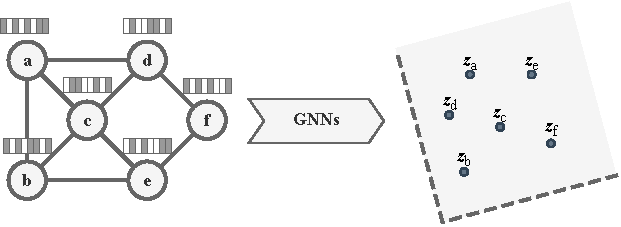
\includegraphics[
                width=0.8\linewidth,
                trim=0pt 0pt 0pt 0pt, % trim: left bottom right top
                clip
            ]{../images/graph_neural_networks.pdf}
            \caption{GNNs scheme.}
            % \source{}
            % \label{fig:my_image}
        \end{figure}

        \begin{note}
            {Introduce your self}
        \end{note}
    \end{frame}

    \begin{frame}{Base GNN models}
        \begin{itemize}
            \item \texttt{VGAE}: Variational graph auto-encoders \cite{kipf2016variational}
            \item \texttt{ARGVA}: Adversarially regularized graph autoencoder for graph embedding \cite{pan2018adversarially}
            \item \texttt{DGI}: Deep graph infomax \cite{velickovic2018deep}
            \item \texttt{LVGAE} Simple and effective graph autoencoders with one-hop linear models \cite{salha2020simple}
            \item \texttt{T-GAE}: Transferable Graph Autoencoder for Network Alignment \cite{he2024t}.
        \end{itemize}

        \begin{note}
            {Introduce your self}
        \end{note}
    \end{frame}

\section{Method}
    \begin{frame}{Mass spectrometry data}
        \begin{figure}[htp!]
            \centering
            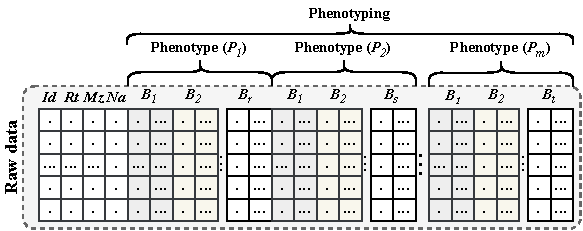
\includegraphics[
                width=0.8\linewidth,
                trim=0pt 0pt 0pt 0pt, % trim: left bottom right top
                clip
            ]{../images/raw_data.pdf}
            \caption{Dataset format.}
            % \source{Author, 2024.}
            % \label{fig:my_image}
        \end{figure}

        \begin{note}
            {Introduce your self}
        \end{note}
    \end{frame}

    \begin{frame}{Approach 1 (matabolomics changes)}
        \begin{columns}[t] % Option "c" centers vertically, while "t" aligns to the top.
            \begin{column}{0.45\textwidth}
                \begin{figure}[htp!]
                    \centering
                    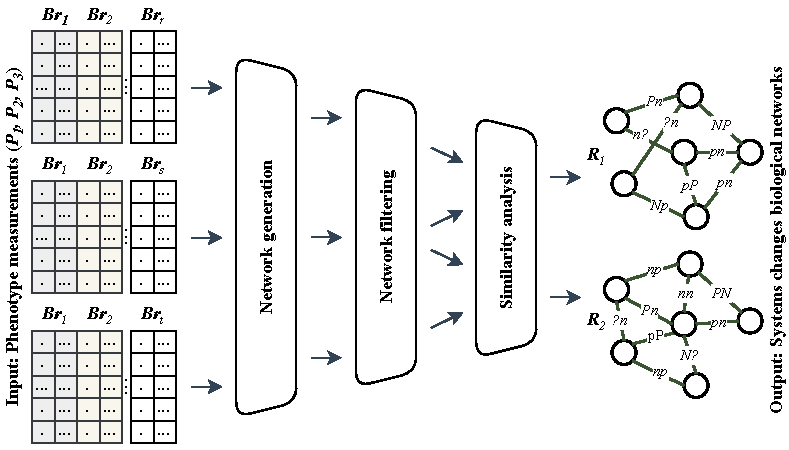
\includegraphics[
                        width=1.0\linewidth,
                        trim=0pt 0pt 0pt 0pt, % trim: left bottom right top
                        clip
                    ]{../images/method_1.pdf}
                    \caption{Our workflow.}
                    % \source{Author, 2024.}
                    % \label{fig:my_image}
                \end{figure}
            \end{column}
            \begin{column}{0.55\textwidth}
                \begin{figure}[htp!]
                    \centering
                    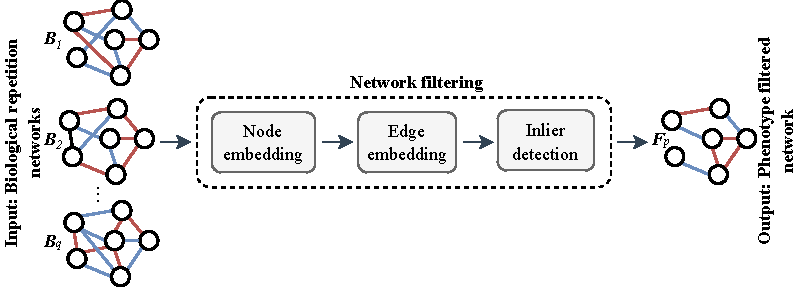
\includegraphics[
                        width=1.0\linewidth,
                        trim=0pt 0pt 0pt 0pt, % trim: left bottom right top
                        clip
                    ]{../images/pipeline2.pdf}
                    \caption{Network filtering.}
                    % \source{Author, 2024.}
                    % \label{fig:my_image}
                \end{figure}
            \end{column}
        \end{columns}

        \begin{note}
            {Introduce your self}
        \end{note}
    \end{frame}

    \begin{frame}{Approach 1}
        \begin{figure}
            \centering
            \begin{subfigure}{0.3\textwidth}
                \centering
                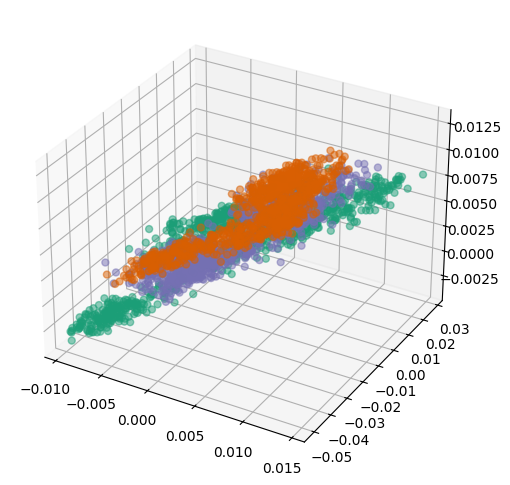
\includegraphics[
                    width=\linewidth,
                    trim=0pt 0pt 0pt 0pt, % trim: left bottom right top
                    clip
                ]{../images/node_embeddings_x.png}
                \caption{Node embeddings.}
                % \source{Author, 2024.}
            \end{subfigure}
            \hfill
            % \hspace{1cm}
            \begin{subfigure}{0.3\textwidth}
                \centering
                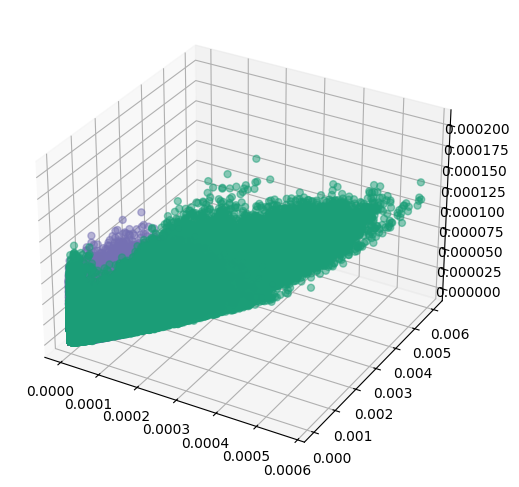
\includegraphics[
                    width=\linewidth,
                    trim=0pt 0pt 0pt 0pt, % trim: left bottom right top
                    clip
                ]{../images/edge_embedding_x.png}
                \caption{Edge embeddings.}
                % \source{Author, 2024.}
            \end{subfigure}
            \hfill
            %\hspace{1cm}
            \begin{subfigure}{0.3\textwidth}
                \centering
                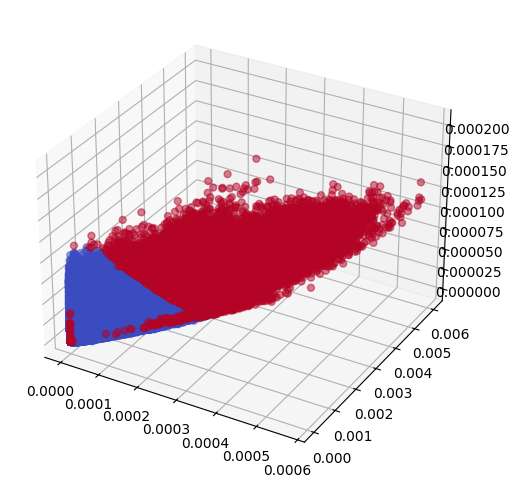
\includegraphics[
                    width=\linewidth,
                    trim=0pt 0pt 0pt 0pt, % trim: left bottom right top
                    clip
                ]{../images/outliers_x.png}
                \caption{Outliers.}
                % \source{Author, 2024.}
            \end{subfigure}
            \caption{Embeddings manipulation for \textit{Warming-treated} phenotype on the Leaf.}
            % \source{Author, 2024.}
            % \label{fig:my_image}
        \end{figure}

        \begin{note}
            {Introduce your self}
        \end{note}
    \end{frame}

    \begin{frame}{Approach 2 (network alignment)}
        \begin{figure}[htp!]
            \centering
            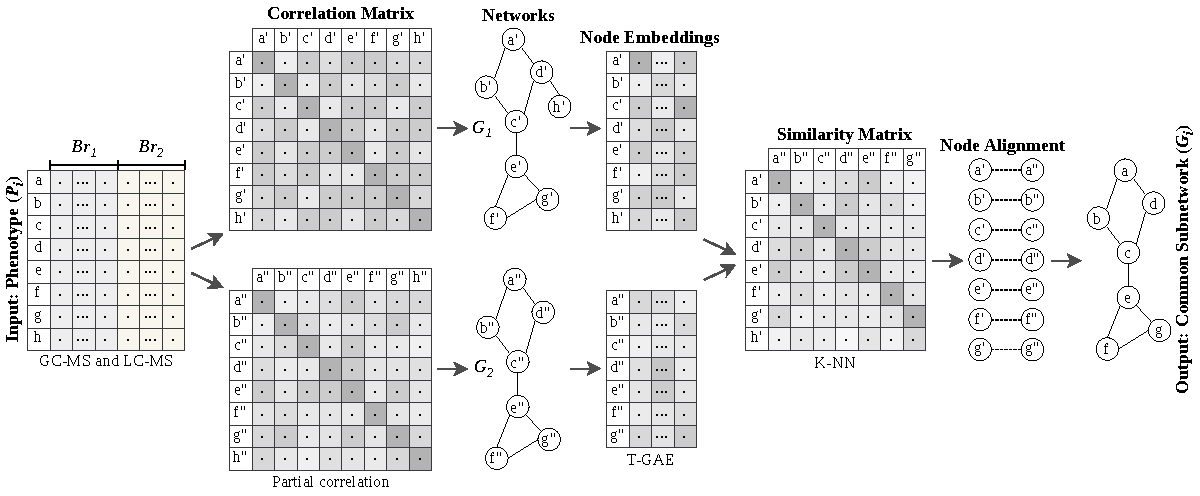
\includegraphics[
                width=1.0\linewidth,
                trim=0pt 0pt 0pt 0pt, % trim: left bottom right top
                clip
            ]{../images/Method_NA.pdf}
            \caption{Our workflow.}
            % \source{Author, 2024.}
            % \label{fig:my_image}
        \end{figure}

        \begin{note}
            {Introduce your self}
        \end{note}
    \end{frame}

    \begin{frame}{Approach 2}
        \begin{figure}
            \centering
            \begin{subfigure}{0.45\textwidth}
                \centering
                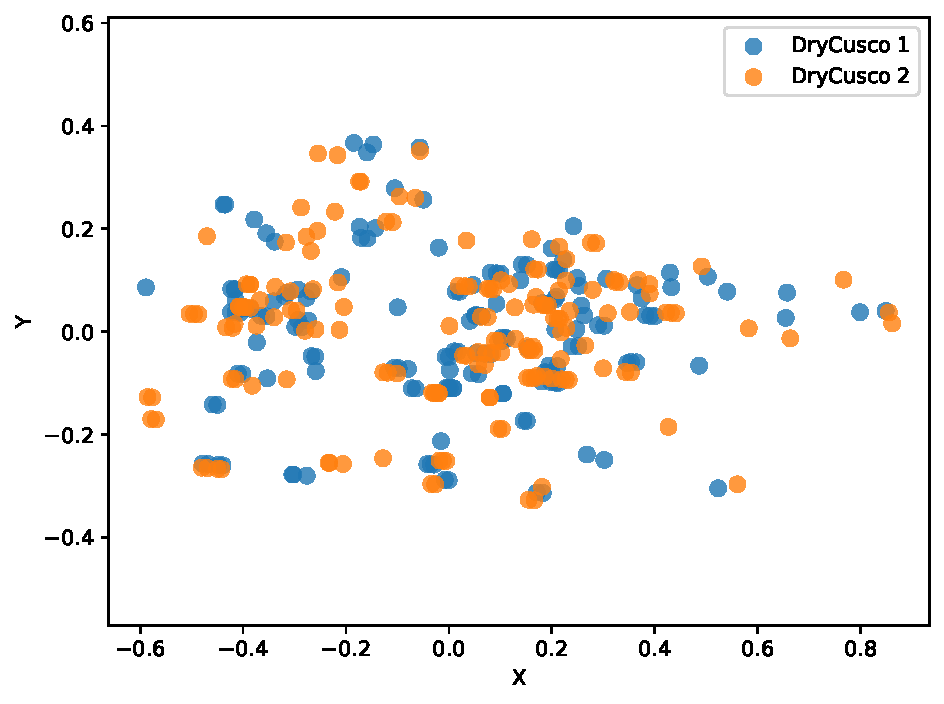
\includegraphics[
                    width=\linewidth,
                    trim=0pt 0pt 0pt 0pt, % trim: left bottom right top
                    clip
                ]{../images/node_embeddings_2d_GINE_SecoCusco.pdf}
                \caption{For Cocoa (DryCusco).}
                % \source{Author, 2024.}
            \end{subfigure}
            % \hfill
            \hspace{1cm}
            \begin{subfigure}{0.4\textwidth}
                \centering
                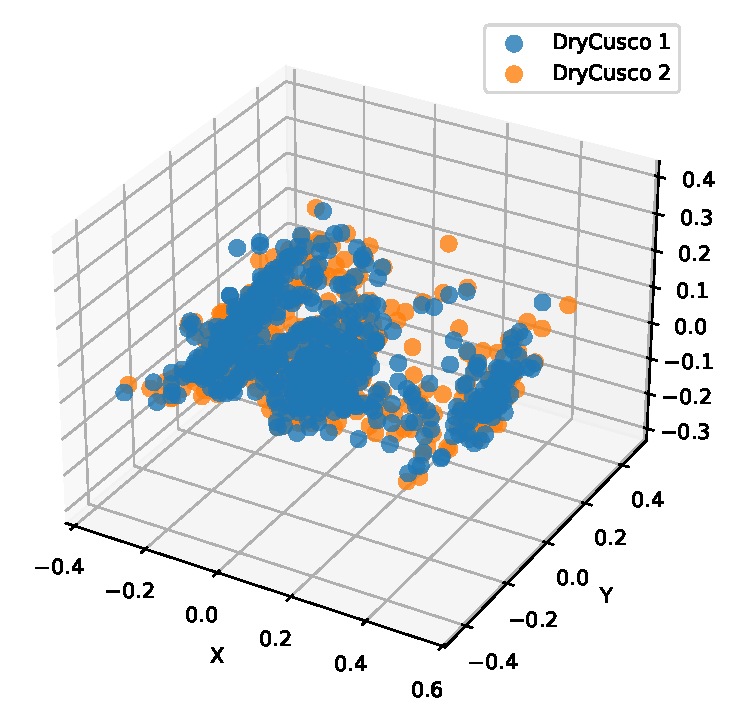
\includegraphics[
                    width=\linewidth,
                    trim=0pt 0pt 0pt 0pt, % trim: left bottom right top
                    clip
                ]{../images/node_embeddings_3d_GINE_SecoCusco.pdf}
                \caption{For Cocoa (DryCusco).}
                % \source{Author, 2024.}
            \end{subfigure}
            \caption{Embeddings manipulation.}
            % \source{Author, 2024.}
            % \label{fig:my_image}
        \end{figure}

        \begin{note}
            {Introduce your self}
        \end{note}
    \end{frame}

\section{Experiments and Results}
    \begin{frame}{Datasets}
        These 5 datasets were used in the experiments. \\
        
        \begin{itemize}
            % \item Synthetic
            \item Mutant \cite{buettner2017non}
            \item Leaf \cite{gonzalez2023climate}
            \item Mentos \cite{alvarez2024exploratory}
            \item Cacao (from ICOBA-PUCP)
            \item Synthetic
        \end{itemize}

        % \begin{table}[htp!]
        %     % \scriptsize
        %     \centering
        %     \caption{Datasets.}
        %     % \label{tab:table1}
        %     \begin{tabular}{@{}llrrrr@{}}
        %         \toprule
        %         Dataset & Type network & \#Nodes  & \#Edges & \#Features & \#Anchors/Pairs \\
        %         \midrule
        %         Douban Online & Social    & $3\,906$ & $1\,632$ & $538$ & $1\,118$  \\
        %         Douban Offline & Social    & $1\,118$   & $3\,022$  & $538$ & $1\,118$ \\\midrule
        %         ACM & Citation  & $9\,916$ & $44\,808$ & $17$ & $6\,325$  \\
        %         DBLP & Citation  & $9\,872$ & $39\,561$  & $17$ & $6\,325$  \\\bottomrule 
        %     \end{tabular}
        % \end{table}

        \begin{note}
            {Introduce your self}
        \end{note}
    \end{frame}

    % \begin{frame}{Experiments setup}

    %     \begin{table}[htp!]
    %         % \scriptsize
    %         \centering
    %         \caption{Experiments setup.}
    %         % \label{tab:table1}
    %         \begin{tabular}{@{}ll@{}}\toprule
    %             Features & Values \\\midrule
    %             Node embedding & 
    %             \texttt{T-GAE} \\
    %             Architectures & \texttt{GIN}, \texttt{GINE} \\
    %             Dimensions & 16, 32, 64 \\ %, 256, 512 \\
    %             Optimizer & Adam with $lr=10^{-4}$, $weight\_decay=5 \times 10^{-4}$ \\
    %             Early stopping & $patience=10$ \\
    %             Epochs & 100 \\\midrule
    %             Node features & $Mz$, $Rt$, $\operatorname{log}(Avg\; intensities)$, $Std\; intensities$, $Cv\; intensities$ \\
    %             Edge features & $|\rho_{ij}|$, $\operatorname{sign}(\rho_{ij})$, $\rho_{ij}^{2}$ \\\midrule
    %             Dataset & Cacao, Leaf, Mentos \\\bottomrule
    %         \end{tabular}
    %     \end{table}

    %     \begin{note}
    %         {Introduce your self}
    %     \end{note}
    % \end{frame}

\section{Results}
    \begin{frame}{Approach 1}
        \begin{figure}[htp!]
            \centering
            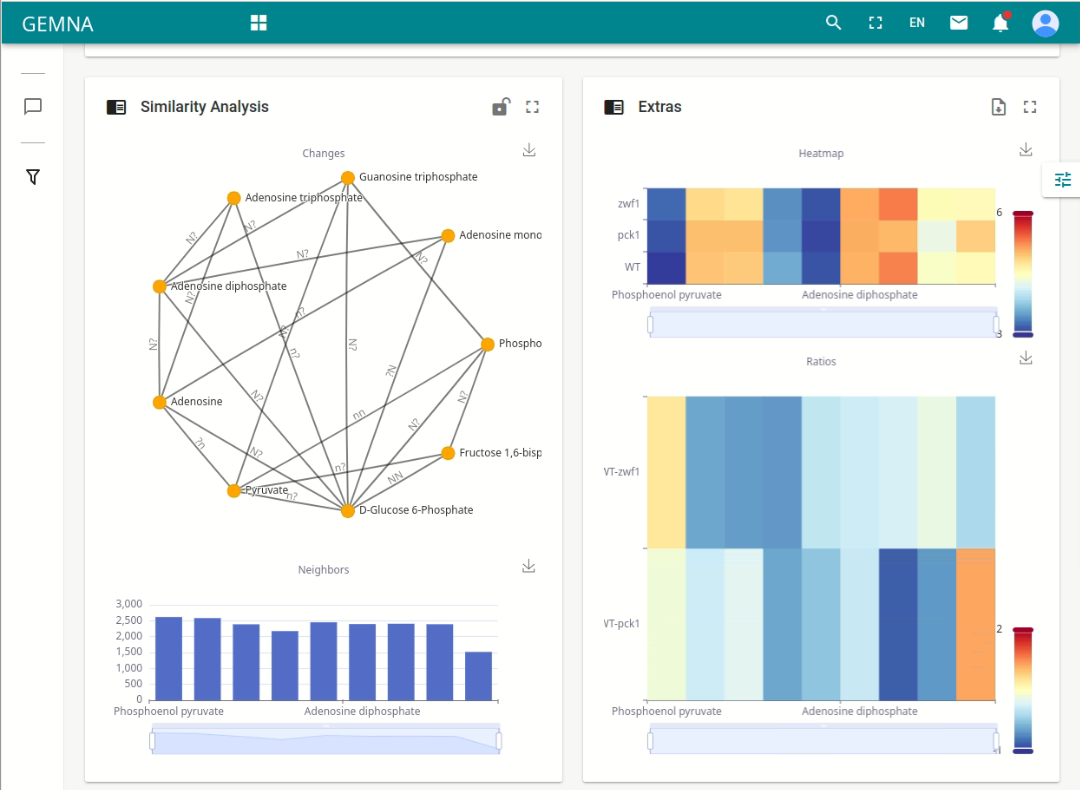
\includegraphics[
                width=0.63\linewidth,
                trim=0pt 0pt 0pt 0pt, % trim: left bottom right top
                clip
            ]{../images/similarity_heatmap.png}
            \caption{Visualization of analysis MS data.}
            % \source{Author, 2024.}
            % \label{fig:my_image}
        \end{figure}

        \begin{note}
            {Introduce your self}
        \end{note}
    \end{frame}

    \begin{frame}{Approach 2}
        \begin{columns}[t] % Option "c" centers vertically, while "t" aligns to the top.
            \begin{column}{0.4\textwidth}
                \begin{table}[htp!]
                    \scriptsize
                    \centering
                    \caption{Node aligment (DryCusco).}
                    % \label{tab:table1}
                    \begin{tabular}{rl}\toprule
                        ID 1 & ID 2 \\\midrule                        
                        0 & 93 \\
                        \rowcolor{yellow}
                        2 & 2 \\
                        4 & 57 \\
                        \rowcolor{yellow}
                        5 & 5 \\
                        7 & 93 \\
                        ... & ... \\
                        \rowcolor{yellow}
                        542 & 542 \\
                        \rowcolor{yellow}
                        551 & 551 \\
                        556 & 509 \\
                        557 & 550 \\
                        558 & 530 \\\bottomrule
                    \end{tabular}
                \end{table}
            \end{column}
            
            \begin{column}{0.6\textwidth}
                \begin{table}[htp!]
                    \scriptsize
                    \centering
                    \caption{Node filtered \textbf{294/559} (DryCusco).}
                    % \label{tab:table1}
                    \begin{tabular}{lrrl}\toprule
                        ID & Rt & Mz & Metabolite name \\\midrule
                        2	& 0.097	& 172.95681 & Unknown \\
                        5	& 0.201	& 144.98254 & Unknown \\
                        15	& 1.871	& 118.08675 & Betaine \\
                        30	& 1.949	& 446.88860 & Unknown \\
                        % 32	& 2.020	& 151.03559 & [Similar to: N-Acetyl-L-cysteine; ΔMass: -13.0... \\
                        % 38	& 2.086	& 381.08003 & 5-({[3-chloro-5-(trifluoromethyl)-2-pyridyl]me... \\
                        46 &	2.110	& 118.08671	& Betaine \\
                        531	& 29.792	& 374.30350 & Docosahexaenoic acid ethyl ester \\
                        532	& 29.794	& 352.32167 & Unknown \\
                        537	& 29.838	& 454.42642 & N-Hexacosanoylglycine \\
                        538	& 29.839	& 150.12816 & 2,6-Diethylaniline \\
                        542	& 29.860	& 398.23344 & Drotaverine \\
                        551	& 29.954	& 150.12807 & 2,6-Diethylaniline \\\bottomrule
                    \end{tabular}
                \end{table}
            \end{column}
        \end{columns}

        \begin{note}
            {Introduce your self}
        \end{note}
    \end{frame}

    % \begin{frame}{Clustering analysis}
    %     \begin{figure}[htp!]
    %         \centering
    %         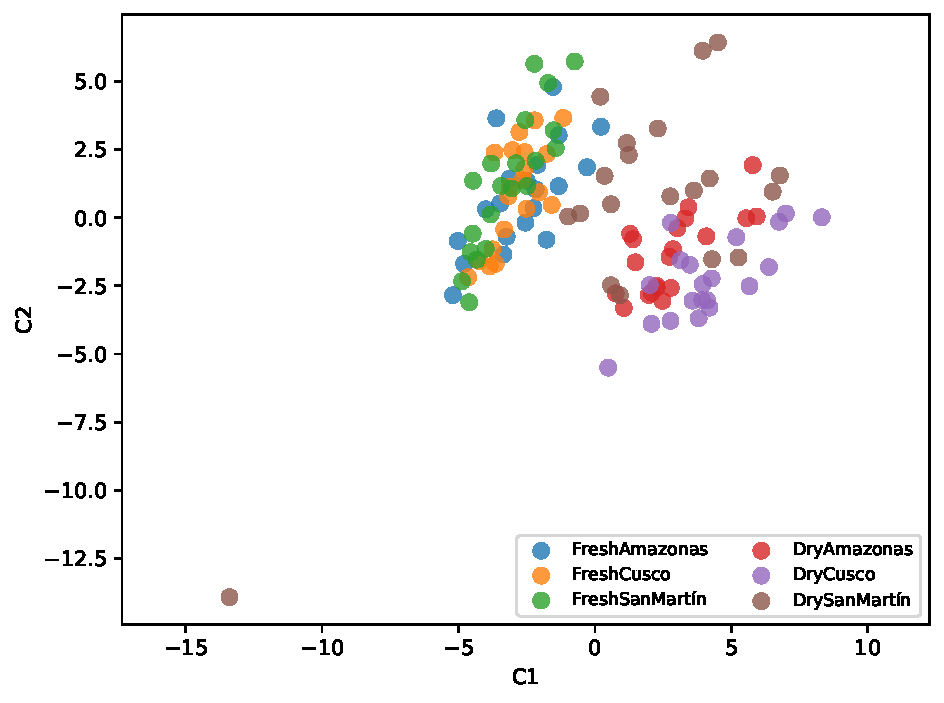
\includegraphics[
    %             width=0.5\linewidth,
    %             trim=0pt 0pt 0pt 0pt, % trim: left bottom right top
    %             clip
    %         ]{../images/clustering_GINE_SecoCusco.pdf}
    %         \caption{Clustering (DryCusco).}
    %         % \source{Author, 2024.}
    %         % \label{fig:my_image}
    %     \end{figure}

    %     \begin{note}
    %         {Introduce your self}
    %     \end{note}
    % \end{frame}

    % \begin{frame}{Comparison of encoders}
    %     \begin{figure}[htp!]
    %         \centering
    %         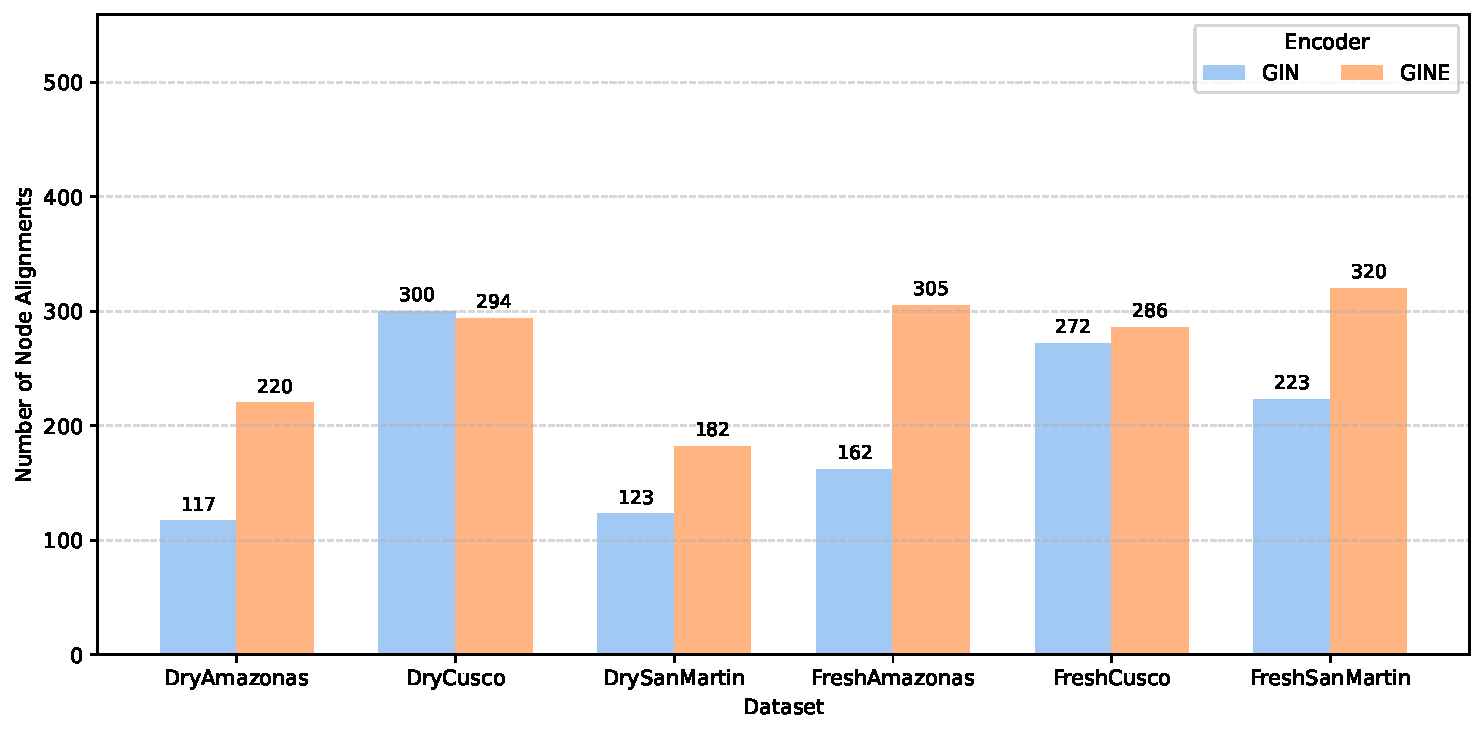
\includegraphics[
    %             width=0.8\linewidth,
    %             trim=0pt 0pt 0pt 0pt, % trim: left bottom right top
    %             clip
    %         ]{../images/number_node_alignment.pdf}
    %         \caption{\texttt{GIN} vs. \texttt{GINE}.}
    %         % \source{Author, 2024.}
    %         % \label{fig:my_image}
    %     \end{figure}

    %     \begin{note}
    %         {Introduce your self}
    %     \end{note}
    % \end{frame}

    % Clustering analysis
    % exp5
    % gine fresco cusco
    % gine seco cusco

\section{Future works}
    \begin{frame}{What is next?}
        \begin{columns}[c] % Option "c" centers vertically, while "t" aligns to the top.
            \begin{column}{0.62\textwidth}
                \begin{itemize}
                    \item Perform exhaustive experiments.
                    \item Model metabolomic networks as signed networks.
                    \item Develop a web application.
                \end{itemize}
            \end{column}
            \begin{column}{0.38\textwidth}
                \begin{figure}[htp!]
                    \centering
                    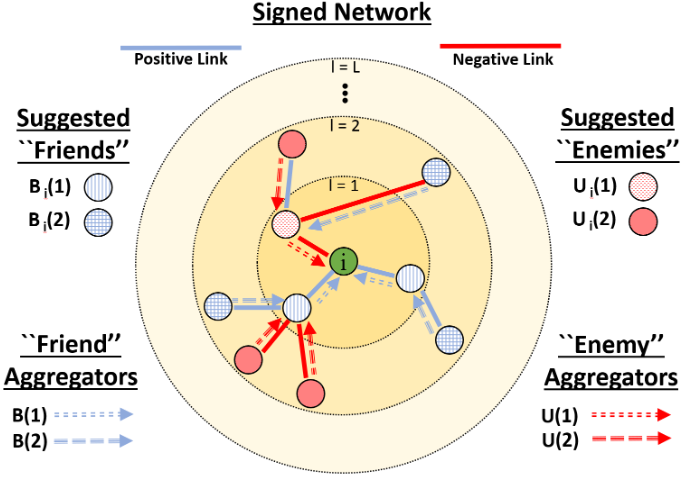
\includegraphics[
                        width=1.0\linewidth,
                        trim=0pt 0pt 0pt 0pt, % trim: left bottom right top
                        clip
                    ]{../images/SGCN.png}
                    \caption{Signed graph convolutional network (SGCN) \cite{derr2018signed}.}
                    % \source{Author, 2024.}
                    % \label{fig:my_image}
                \end{figure}
            \end{column}
        \end{columns}

        \begin{note}
            {Introduce your self}
        \end{note}
    \end{frame}


% \section{Conclusions}
%     \begin{frame}{Conclusions}
%         Our proposal, is a approach to the exploratory analysis of metabolic networks.

%         % Features
%         \begin{itemize}
%             % Significant, noise
%             \item Features shared by cacao beans within the same group are retained, reducing the number of features before identification is attempted.
            
%             % Prediction, inferencial
%             \item A core graph embedding is generated for each cacao bean, providing a compact representation that can be used as input to a classifier for subsequent cacao bean identification.
            
%             % Worflow, improve  (atemporal)
%             \item The alignment workflow enables samples acquired on different days to be integrated into a single dataset. This approach mitigates known batch effects, such as retention-time shifts, while the graph embedding favors correlations among signals rather than depending on their absolute intensity values.
            
%             % \item We designed a pipeline for a metabolomic study. \texttt{GEMNA} consists of three steps: \textit{network generation}, \textit{network filtering}, and \textit{similarity analysis}.

%             % \item We evaluated the execution time for generating node embeddings and edge embeddings. The experiments demonstrate that \texttt{DGI} model is faster than \texttt{VGAE}, \texttt{LVGAE}, \texttt{ARGVA}, to generate node embeddings. % using node embeddings (based on GNN), edge embeddings, and anomaly detection algorithm.

%             % \item Experiments show that our \texttt{GEMNA} is an improvement over traditional statistical-based techniques. The evaluation by silhouette score reported that \texttt{GEMNA} obtained $0.41$, meanwhile, the statistical method obtained $-0.004$. % For example, for the Mentos candy dataset, the data clusters produced by \texttt{GEMNA} were better than the ones used in traditional techniques based on statistics. \texttt{GEMNA} has $silhouette\:score = 0.409$, \textit{vs} the traditional approach has $silhouette\:score = -0.004$.

%             % \item We developed a web application for metabolomic network analysis and the source code is available on GitHub.
%         \end{itemize}

%         \begin{note}
%             {Write your notes here}
%         \end{note}
%     \end{frame}

% % \begin{frame}{Future works}
% %     Based on these results, I recommend analyzing metabolomic networks using \textit{Geometric Graph Neural Networks} (GGNN) models.

% %     These models create node embeddings using the graph structure, node and edge features, and a feature tensor that helps infer the position of each metabolite within the network.
    
% %     \begin{note}
% %         {Write your notes here}
% %     \end{note}
% % \end{frame}

\section*{References}
    % Bibliography
    % \input{ref.bib}
    \begin{frame}[allowframebreaks]
        \footnotesize % use this command to resize
        \bibliography{ref}
        \bibliographystyle{unsrt}
        % \bibliographystyle{alpha}
        
        % \begin{itemize}
        %     \item Erciyes, K. (2018). \textit{Guide to graph algorithms} % (pp. 15-35). Springer International Publishing.
        %     \item Yao Ma, Jiliang Tang. (2021). \textit{Deep Learning on Graphs}.
        %     \item Stamile C., Marzullo A., Deusebio E. (2021). \textit{Graph Machine Learning}.
        %     \item Wu, L., Cui, P., Pei, J., Zhao, L., \& Guo, X. (2022). \textit{Graph neural networks: foundation, frontiers and applications}. % In Proceedings of the 28th ACM SIGKDD conference on knowledge discovery and data mining (pp. 4840-4841).            
        %     % \item Knickerbocker D. (2023). \textit{Graph Network Science with Python}.
        %     \item Knickerbocker, D. (2023). \textit{Network Science with Python}. % Packt Publishing Ltd.
        %     \item Labonne, M. (2023). \textit{Hands-On Graph Neural Networks Using Python}.
        %     \item Broadwater, K., \& Stillman, N. (2025). \textit{Graph neural networks in action}. % Simon and Schuster.
        % \end{itemize}
    \end{frame}

    \begin{frame}
        \begin{center}
            {\Huge\calligra Thanks!} \\
            % {\Huge\textit{Thank you for your attention!}}\\
            {\Huge $\infty$} \\
            edwin.alvarez@pucp.edu.pe \\
            \url{https://github.com/win7}
        \end{center}
    \end{frame}
\end{document}